\documentclass[11pt,letterpaper]{article}
\usepackage{graphicx}
\usepackage[left=3cm,top=2cm,bottom=2cm,right=3cm]{geometry}
\usepackage[title,titletoc]{appendix}
\usepackage[noblocks]{authblk}
%\usepackage{multirow}
\usepackage{url}
\usepackage{subfigure}
\usepackage{draftwatermark}

% The default is to indent the start of each paragraph.  This is
% annoying and we can disable it with this:
% \setlength\parindent{0pt}

\title{\bf Data Formatter Firmware Design Note}
\author{Yasuyuki Okumura}
\affil{University of Chicago, Chicago, Illinois 60637, USA}
\author{Zihao Jiang}
\affil{Stanford University, Stanford, California, 94305, USA}
\date{\today}

% watermark DRAFT on each page
\SetWatermarkLightness{ 0.95 }
\SetWatermarkScale{ 5 }

\begin{document}
\maketitle

\begin{abstract}
\end{abstract}

\section{Introduction}
This describes the design of the Data Formatter Firmware. The documentation is for GitHub revision of \url{data_formatter_firmware-00-00-03}. This version of firmware is developed from \url{data_formatter_firmware-00-00-02} branch. All the needed details can be found in the \url{DF_Design_V00-00-03-branch.xlsx}, too.

\section{Changes of this version of FW}
This version of FW includes the following significant changes:
\begin{enumerate}
 \item Implementation of IM-DF block transfer 
 \item Implementation of automatic FMC delay value setting
 \item Bug fix for SPY buffer inconsistent readout
 \item Bug fix for AUX-DF slink communication (AUX idle words as pad words, partially done)
 \item Addition of registers to read out fmc fifo fullness, fmc fifo number of words writte, FW version and etc.
 \item Addition of SLINK output for SSB and implementation of QSFP link for inter-crate DF communication and DF-SSB communication
 \item Addition of the functionality to change IP address for FW through IPBus
\end{enumerate}


\section{32 board allocation and numbering}

Table \ref{tab:shelf1}, \ref{tab:shelf2}, \ref{tab:shelf3} and \ref{tab:shelf4} show DF boards allocation and numbering in USA 15. 

\begin{table}[h]
\tiny
\begin{tabular}{|c|c|c|c|c|c|c|c|c|c|}
\hline
Board ID               & bit mask              & \multicolumn{2}{c|}{location}                          & \multicolumn{2}{c|}{destination 1}                            & \multicolumn{2}{c|}{destination 2}                            & \multicolumn{2}{c|}{inter-crate link destination} \\ \hline
\multicolumn{1}{|l|}{} & \multicolumn{1}{l|}{} & \multicolumn{1}{l|}{Shelf} & \multicolumn{1}{l|}{Slot} & \multicolumn{1}{l|}{Tower ID} & \multicolumn{1}{l|}{Position} & \multicolumn{1}{l|}{Tower ID} & \multicolumn{1}{l|}{Position} & Link 1                  & Link 2                  \\ \hline
0                      & 0x00000001            & 1                          & 3                         & 2                             & C E phi1                      & 3                             & C E phi2                      & Shelf 4 - Slot 7        & Shelf 2 - Slot 7        \\ \hline
4                      & 0x00000010            & 1                          & 4                         & 18                            & C B phi1                      & 19                            & C B phi2                      & Shelf 4 - Slot 8        & Shelf 2 - Slot 8        \\ \hline
8                      & 0x00000100            & 1                          & 5                         & 34                            & A B phi1                      & 35                            & A B phi2                      & Shelf 4 - Slot 9        & Shelf 2 - Slot 9        \\ \hline
12                     & 0x00001000            & 1                          & 6                         & 50                            & A E phi1                      & 51                            & A E phi2                      & Shelf 4 - Slot 10       & Shelf 2 - Slot 10       \\ \hline
16                     & 0x00010000            & 1                          & 7                         & 4                             & C E phi3                      & 5                             & C E phi4                      & Shelf 4 - Slot 3        & Shelf 2 - Slot 3        \\ \hline
20                     & 0x00100000            & 1                          & 8                         & 20                            & C B phi3                      & 21                            & C B phi4                      & Shelf 4 - Slot 4        & Shelf 2 - Slot 4        \\ \hline
24                     & 0x01000000            & 1                          & 9                         & 36                            & A B phi3                      & 37                            & A B phi4                      & Shelf 4 - Slot 5        & Shelf 2 - Slot 5        \\ \hline
28                     & 0x10000000            & 1                          & 10                        & 52                            & A E phi3                      & 53                            & A E phi4                      & Shelf 4 - Slot 6        & Shelf 2 - Slot 6        \\ \hline
\end{tabular}
\caption{Shelf 1.}
\label{tab:shelf1}
\end{table}

\begin{table}[h]
\tiny
\begin{tabular}{|c|c|c|c|c|c|c|c|c|c|}
\hline
Board ID               & bit mask              & \multicolumn{2}{c|}{location}                          & \multicolumn{2}{c|}{destination 1}                            & \multicolumn{2}{c|}{destination 2}                            & \multicolumn{2}{c|}{inter-crate link destination} \\ \hline
\multicolumn{1}{|l|}{} & \multicolumn{1}{l|}{} & \multicolumn{1}{l|}{Shelf} & \multicolumn{1}{l|}{Slot} & \multicolumn{1}{l|}{Tower ID} & \multicolumn{1}{l|}{Position} & \multicolumn{1}{l|}{Tower ID} & \multicolumn{1}{l|}{Position} & Link 1                  & Link 2                  \\ \hline
1                      & 0x00000002            & 2                          & 3                         & 6                             & C E phi5                      & 7                             & C E phi6                      & Shelf 1 - Slot 7        & Shelf 3 - Slot 7        \\ \hline
5                      & 0x00000020            & 2                          & 4                         & 22                            & C B phi5                      & 23                            & C B phi6                      & Shelf 1 - Slot 8        & Shelf 3 - Slot 8        \\ \hline
9                      & 0x00000200            & 2                          & 5                         & 38                            & A B phi5                      & 39                            & A B phi6                      & Shelf 1 - Slot 9        & Shelf 3 - Slot 9        \\ \hline
13                     & 0x00002000            & 2                          & 6                         & 54                            & A E phi5                      & 55                            & A E phi6                      & Shelf 1 - Slot 10       & Shelf 3 - Slot 10       \\ \hline
17                     & 0x00020000            & 2                          & 7                         & 8                             & C E phi7                      & 9                             & C E phi8                      & Shelf 1 - Slot 3        & Shelf 3 - Slot 3        \\ \hline
21                     & 0x00200000            & 2                          & 8                         & 24                            & C B phi7                      & 25                            & C B phi8                      & Shelf 1 - Slot 4        & Shelf 3 - Slot 4        \\ \hline
25                     & 0x02000000            & 2                          & 9                         & 40                            & A B phi7                      & 41                            & A B phi8                      & Shelf 1 - Slot 5        & Shelf 3 - Slot 5        \\ \hline
29                     & 0x20000000            & 2                          & 10                        & 53                            & A E phi7                      & 54                            & A E phi8                      & Shelf 1 - Slot 6        & Shelf 3 - Slot 6        \\ \hline
\end{tabular}
\caption{Shelf 2.}
\label{tab:shelf2}
\end{table}

\begin{table}[h]
\tiny
\begin{tabular}{|c|c|c|c|c|c|c|c|c|c|}
\hline
Board ID               & bit mask              & \multicolumn{2}{c|}{location}                          & \multicolumn{2}{c|}{destination 1}                            & \multicolumn{2}{c|}{destination 2}                            & \multicolumn{2}{c|}{inter-crate link destination} \\ \hline
\multicolumn{1}{|l|}{} & \multicolumn{1}{l|}{} & \multicolumn{1}{l|}{Shelf} & \multicolumn{1}{l|}{Slot} & \multicolumn{1}{l|}{Tower ID} & \multicolumn{1}{l|}{Position} & \multicolumn{1}{l|}{Tower ID} & \multicolumn{1}{l|}{Position} & Link 1                  & Link 2                  \\ \hline
2                      & 0x00000004            & 3                          & 3                         & 10                            & C E phi9                      & 11                            & C E phi10                     & Shelf 2 - Slot 7        & Shelf 4 - Slot 7        \\ \hline
6                      & 0x00000040            & 3                          & 4                         & 26                            & C B phi9                      & 27                            & C B phi10                     & Shelf 2 - Slot 8        & Shelf 4 - Slot 8        \\ \hline
10                     & 0x00000400            & 3                          & 5                         & 42                            & A B phi9                      & 43                            & A B phi10                     & Shelf 2 - Slot 9        & Shelf 4 - Slot 9        \\ \hline
14                     & 0x00004000            & 3                          & 6                         & 58                            & A E phi9                      & 59                            & A E phi10                     & Shelf 2 - Slot 10       & Shelf 4 - Slot 10       \\ \hline
18                     & 0x00040000            & 3                          & 7                         & 12                            & C E phi11                     & 13                            & C E phi12                     & Shelf 2 - Slot 3        & Shelf 4 - Slot 3        \\ \hline
22                     & 0x00400000            & 3                          & 8                         & 28                            & C B phi11                     & 29                            & C B phi12                     & Shelf 2 - Slot 4        & Shelf 4 - Slot 4        \\ \hline
26                     & 0x04000000            & 3                          & 9                         & 44                            & A B phi11                     & 45                            & A B phi12                     & Shelf 2 - Slot 5        & Shelf 4 - Slot 5        \\ \hline
30                     & 0x40000000            & 3                          & 10                        & 60                            & A E phi11                     & 61                            & A E phi12                     & Shelf 2 - Slot 6        & Shelf 4 - Slot 6        \\ \hline
\end{tabular}
\caption{Shelf 3.}
\label{tab:shelf3}
\end{table}

\begin{table}[h]
\tiny
\begin{tabular}{|c|c|c|c|c|c|c|c|c|c|}
\hline
Board ID               & bit mask              & \multicolumn{2}{c|}{location}                          & \multicolumn{2}{c|}{destination 1}                            & \multicolumn{2}{c|}{destination 2}                            & \multicolumn{2}{c|}{inter-crate link destination} \\ \hline
\multicolumn{1}{|l|}{} & \multicolumn{1}{l|}{} & \multicolumn{1}{l|}{Shelf} & \multicolumn{1}{l|}{Slot} & \multicolumn{1}{l|}{Tower ID} & \multicolumn{1}{l|}{Position} & \multicolumn{1}{l|}{Tower ID} & \multicolumn{1}{l|}{Position} & Link 1                  & Link 2                  \\ \hline
3                      & 0x00000008            & 4                          & 3                         & 14                            & C E phi13                     & 15                            & C E phi14                     & Shelf 3 - Slot 7        & Shelf 1 - Slot 7        \\ \hline
7                      & 0x00000080            & 4                          & 4                         & 30                            & C B phi13                     & 31                            & C B phi14                     & Shelf 3 - Slot 8        & Shelf 1 - Slot 8        \\ \hline
11                     & 0x00000800            & 4                          & 5                         & 46                            & A B phi13                     & 47                            & A B phi14                     & Shelf 3 - Slot 9        & Shelf 1 - Slot 9        \\ \hline
15                     & 0x00008000            & 4                          & 6                         & 62                            & A E phi13                     & 63                            & A E phi14                     & Shelf 3 - Slot 10       & Shelf 1 - Slot 10       \\ \hline
20                     & 0x00080000            & 4                          & 7                         &  0                            & C E phi15                     &  1                            & C E phi0                      & Shelf 3 - Slot 3        & Shelf 1 - Slot 3        \\ \hline
24                     & 0x00800000            & 4                          & 8                         & 16                            & C B phi15                     & 17                            & C B phi0                      & Shelf 3 - Slot 4        & Shelf 1 - Slot 4        \\ \hline
27                     & 0x08000000            & 4                          & 9                         & 32                            & A B phi15                     & 33                            & A B phi0                      & Shelf 3 - Slot 5        & Shelf 1 - Slot 5        \\ \hline
31                     & 0x80000000            & 4                          & 10                        & 48                            & A E phi15                     & 49                            & A E phi0                      & Shelf 3 - Slot 6        & Shelf 1 - Slot 6        \\ \hline
\end{tabular}
\caption{Shelf 4.}
\label{tab:shelf4}
\end{table}

\clearpage

\section{Overview of the firmware}

\begin{figure}[h!]
  \centering
  \includegraphics[width=0.80\textwidth,clip,page=3]{figures.pdf}
  \caption{Firmware overview.}
  \label{fig:OVERVIEW}
\end{figure}

\section{Main logic}
\begin{itemize}
\item FMC interface : \url{data_formatter_top/df_fmc_interface.vhd}
\item Input data operator : \url{data_formatter_top/df_input_data_operator.vhd}
\item Output data operator : \url{data_formatter_top/df_output_data_operator_v2.vhd}
\item Internal Link input : \url{data_formatter_top/df_internallink_input.vhd}
\item Internal Link input : \url{data_formatter_top/df_internallink_output.vhd}
\end{itemize}

\begin{figure}[h!]
  \centering
  \includegraphics[width=0.95\textwidth,clip,page=4]{figures.pdf}
  \caption{Main logic overview.}
  \label{fig:MAIN_LOGIC_OVERVIEW}
\end{figure}

\subsection{FMC interface}
\begin{itemize}
\item Input mapper : \url{pulsar2_fmc_interface/fmc_rx_mapper_fmc_to_fpga.vhd}
\item Front : \url{pulsar2_fmc_interface/fmc_rx_front.vhd}
\item Mapper : \url{pulsar2_fmc_interface/fmc_rx_mapper_fpga_to_detword.vhd}
\item Parity checker : \url{pulsar2_fmc_interface/fmc_rx_parity.vhd}
\item Frame : \url{pulsar2_fmc_interface/fmc_rx_frame.vhd}
\item Pattern checker : \url{pulsar2_fmc_interface/fmc_rx_data_checker_v3.vhd}
\item Elasitc buffer : \url{fmc_input_buffer/fmc_input_buffer.vhd}
\item FMC TX interface : \url{pulsar2_fmc_interface/fmc_tx_interface.vhd}
\end{itemize}

\begin{figure}[h!]
  \centering
  \includegraphics[width=0.95\textwidth,clip,page=5]{figures.pdf}
  \caption{FMC interface firmware overview.}
  \label{fig:FMC_INTERFACE_OVERVIEW}
\end{figure}

\subsection{Input data operator}

\begin{itemize}
\item Input lane handler : \url{pulsar2_df_internal_decoder/df_input_handler.vhd}
\item Internal frame adder : \url{pulsar2_df_internal_decoder/add_df_internalframe.vhd}
\item SWITCH : \url{pulsar2_df_switch/df_switch_element_v3.vhd}
\end{itemize}

\begin{figure}[h!]
  \centering
  \includegraphics[width=0.95\textwidth,clip,page=6]{figures.pdf}
  \caption{Internal data operator. One modules have three additional words, header, destination words and trailer.}
  \label{fig:INTERNAL_DATA_FORMAT}
\end{figure}

\begin{figure}[h!]
  \centering
  \includegraphics[width=0.95\textwidth,clip,page=7]{figures.pdf}
  \caption{Input data operator firmware overview.}
  \label{fig:INPUT_DATA_OPERATOR_OVERVIEW}
\end{figure}

\begin{figure}[h!]
  \centering
  \includegraphics[width=0.95\textwidth,clip,page=8]{figures.pdf}
  \caption{State machine in Internal frame adder.}
  \label{fig:STATE_MACHINE_FRAME_ADDER}
\end{figure}

\subsection{Output data operator}

\begin{table}[h]
\centering
\begin{tabular}{|c|c|c|c|c|c|c|}
\cline{1-3} \cline{5-7}
lane & \multicolumn{2}{c|}{description} &  & lane & \multicolumn{2}{c|}{description} \\ \cline{1-3} \cline{5-7} 
     & type            & channel        &  &      & type           & channel         \\ \cline{1-3} \cline{5-7} 
0    & IM              & ch0 and ch1    &  & 16   & IM             & ch8 and ch9     \\ \cline{1-3} \cline{5-7} 
1    & Fabric          & ch3 p0         &  & 17   & Fabric         & ch3 p1          \\ \cline{1-3} \cline{5-7} 
2    & Fabric          & ch4 p0         &  & 18   & Fabric         & ch4 p1          \\ \cline{1-3} \cline{5-7} 
3    & Fabric          & ch5 p0         &  & 19   & Fabric         & ch5 p1          \\ \cline{1-3} \cline{5-7} 
4    & IM              & ch2 and ch3    &  & 20   & IM             & ch10 and ch11   \\ \cline{1-3} \cline{5-7} 
5    & Fabric          & ch6 p0         &  & 21   & Fabric         & ch6 p1          \\ \cline{1-3} \cline{5-7} 
6    & Fabric          & ch7 p0         &  & 22   & Fabric         & ch7 p1          \\ \cline{1-3} \cline{5-7} 
7    & Fabric          & ch8 p0         &  & 23   & Fabric         & ch8 p1          \\ \cline{1-3} \cline{5-7} 
8    & IM              & ch4 and ch5    &  & 24   & IM             & ch12 and ch13   \\ \cline{1-3} \cline{5-7} 
9    & Fabric          & ch9 po0        &  & 25   & Fabric         & ch9 p1          \\ \cline{1-3} \cline{5-7} 
10   & Fabric          & ch10 p0        &  & 26   & Fabric         & ch10 p1         \\ \cline{1-3} \cline{5-7} 
11   & Fabric          & ch11 p0        &  & 27   & Fabric         & ch11 p1         \\ \cline{1-3} \cline{5-7} 
12   & IM              & ch6 and ch7    &  & 28   & IM             & ch14 and ch15   \\ \cline{1-3} \cline{5-7} 
13   & Fabric          & ch12 p0        &  & 29   & Fabric         & ch12 p1         \\ \cline{1-3} \cline{5-7} 
14   & Inter-crate     & ch0 p0         &  & 30   & Inter-crate    & ch0 p1          \\ \cline{1-3} \cline{5-7} 
15   & Inter-crate     & ch1 p0         &  & 31   & Inter-crate    & ch1 p1          \\ \cline{1-3} \cline{5-7} 
\end{tabular}
\caption{Input channel assignment for output data operator module. Defined in 
``MAPPING\_CONF\_IDO2ODO'' and ``MAPPING\_CONF\_ILI2ODO'' in data\_formatter\_top/data\_formatter\_constants.vhd.}
\end{table}

\begin{table}[h]
\centering
\begin{tabular}{|c|c|c|c|c|c|c|}
\cline{1-3} \cline{5-7}
lane & \multicolumn{2}{c|}{description} &  & lane & \multicolumn{2}{c|}{description} \\ \cline{1-3} \cline{5-7} 
     & type              & channel      &  &      & type              & channel      \\ \cline{1-3} \cline{5-7} 
0    & AUX0 Tower 0      & ch0          &  & 17   & AUX0 Tower 1      & ch0          \\ \cline{1-3} \cline{5-7} 
1    & AUX0 Tower 0      & ch1          &  & 18   & AUX0 Tower 1      & ch1          \\ \cline{1-3} \cline{5-7} 
2    & AUX0 Tower 0      & ch2          &  & 19   & AUX0 Tower 1      & ch2          \\ \cline{1-3} \cline{5-7} 
3    & AUX0 Tower 0      & ch3          &  & 20   & AUX0 Tower 1      & ch3          \\ \cline{1-3} \cline{5-7} 
4    & AUX1 Tower 0      & ch4          &  & 21   & AUX1 Tower 1      & ch4          \\ \cline{1-3} \cline{5-7} 
5    & AUX1 Tower 0      & ch5          &  & 22   & AUX1 Tower 1      & ch5          \\ \cline{1-3} \cline{5-7} 
6    & AUX1 Tower 0      & ch6          &  & 23   & AUX1 Tower 1      & ch6          \\ \cline{1-3} \cline{5-7} 
7    & AUX1 Tower 0      & ch7          &  & 24   & AUX1 Tower 1      & ch7          \\ \cline{1-3} \cline{5-7} 
8    & AUX2 Tower 0      & ch0          &  & 25   & AUX2 Tower 1      & ch0          \\ \cline{1-3} \cline{5-7} 
9    & AUX2 Tower 0      & ch1          &  & 26   & AUX2 Tower 1      & ch1          \\ \cline{1-3} \cline{5-7} 
10   & AUX2 Tower 0      & ch2          &  & 27   & AUX2 Tower 1      & ch2          \\ \cline{1-3} \cline{5-7} 
11   & AUX2 Tower 0      & ch3          &  & 28   & AUX2 Tower1       & ch3          \\ \cline{1-3} \cline{5-7} 
12   & AUX3 Tower 0      & ch4          &  & 29   & AUX3 Tower1       & ch4          \\ \cline{1-3} \cline{5-7} 
13   & AUX3 Tower 0      & ch5          &  & 30   & AUX3 Tower1       & ch5          \\ \cline{1-3} \cline{5-7} 
14   & AUX3 Tower 0      & ch6          &  & 31   & AUX3 Tower1       & ch6          \\ \cline{1-3} \cline{5-7} 
15   & AUX3 Tower 0      & ch7          &  & 32   & AUX3 Tower 1      & ch7          \\ \cline{1-3} \cline{5-7} 
16   & SSB Tower 0       &              &  & 33   & SSB Tower 1       &              \\ \cline{1-3} \cline{5-7} 
\end{tabular}
\caption{SLINK output channel assignment (34 channel). 
``MAPPING\_CONF\_SLINKOUT2GTLOC'' and ``MAPPING\_CONF\_SLINKOUT2GTLOC'' in data\_formatter\_top/data\_formatter\_constants.vhd.}
\end{table}



\begin{itemize}
\item DF output preparation : \url{pulsar2_df_internal_decoder/df_output_preparation_v2.vhd}
\item Switch 32 x 32 : \url{pulsar2_df_switch/df_switch_matrix_32x32.vhd}
\item Duplicator : \url{pulsar2_df_internal_decoder/df_output_duplicator.vhd}
\item SLINK Packer : \url{pulsar2_df_internal_decoder/df_output_slink_packer_v2.vhd}
\end{itemize}

\begin{figure}[h!]
  \centering
  \includegraphics[width=0.95\textwidth,clip,page=9]{figures.pdf}
  \caption{Output data operator firmware overview.}
  \label{fig:OUTPUT_DATA_OPERATOR_OVERVIEW}
\end{figure}

\begin{figure}[h!]
  \centering
  \includegraphics[width=0.95\textwidth,clip,page=10]{figures.pdf}
  \caption{Schematics of event sorting buffer in the SLINK packer.}
  \label{fig:EVENT_SORTING_BUFFER}
\end{figure}

\subsection{Internal link input / output}

\begin{table}[h]
\centering
\begin{tabular}{|c|c|c|c|c|c|c|}
\cline{1-3} \cline{5-7}
lane & \multicolumn{2}{c|}{description} &  & lane & \multicolumn{2}{c|}{description} \\ \cline{1-3} \cline{5-7} 
     & type            & channel        &  &      & type           & channel         \\ \cline{1-3} \cline{5-7} 
0    & IM              & ch0 and ch1    &  & 16   & IM             & ch8 and ch9     \\ \cline{1-3} \cline{5-7} 
1    & Fabric          & ch3 p0         &  & 17   & Fabric         & ch3 p1          \\ \cline{1-3} \cline{5-7} 
2    & Fabric          & ch4 p0         &  & 18   & Fabric         & ch4 p1          \\ \cline{1-3} \cline{5-7} 
3    & Fabric          & ch5 p0         &  & 19   & Fabric         & ch5 p1          \\ \cline{1-3} \cline{5-7} 
4    & IM              & ch2 and ch3    &  & 20   & IM             & ch10 and ch11   \\ \cline{1-3} \cline{5-7} 
5    & Fabric          & ch6 p0         &  & 21   & Fabric         & ch6 p1          \\ \cline{1-3} \cline{5-7} 
6    & Fabric          & ch7 p0         &  & 22   & Fabric         & ch7 p1          \\ \cline{1-3} \cline{5-7} 
7    & Fabric          & ch8 p0         &  & 23   & Fabric         & ch8 p1          \\ \cline{1-3} \cline{5-7} 
8    & IM              & ch4 and ch5    &  & 24   & IM             & ch12 and ch13   \\ \cline{1-3} \cline{5-7} 
9    & Fabric          & ch9 po0        &  & 25   & Fabric         & ch9 p1          \\ \cline{1-3} \cline{5-7} 
10   & Fabric          & ch10 p0        &  & 26   & Fabric         & ch10 p1         \\ \cline{1-3} \cline{5-7} 
11   & Fabric          & ch11 p0        &  & 27   & Fabric         & ch11 p1         \\ \cline{1-3} \cline{5-7} 
12   & IM              & ch6 and ch7    &  & 28   & IM             & ch14 and ch15   \\ \cline{1-3} \cline{5-7} 
13   & Fabric          & ch12 p0        &  & 29   & Fabric         & ch12 p1         \\ \cline{1-3} \cline{5-7} 
14   & Inter-crate     & ch0 p0         &  & 30   & Inter-crate    & ch0 p1          \\ \cline{1-3} \cline{5-7} 
15   & Inter-crate     & ch1 p0         &  & 31   & Inter-crate    & ch1 p1          \\ \cline{1-3} \cline{5-7} 
\end{tabular}
\caption{Input channel assignment for internal data output module (i.e. input of Central Switch.). Defined in 
``MAPPING\_CONF\_IDO2ILO'' and ``MAPPING\_CONF\_ILI2ILO'' in data\_formatter\_top/data\_formatter\_constants.vhd.}
\end{table}

\begin{table}[h]
\centering
\begin{tabular}{|c|c|c|c|c|c|c|}
\cline{1-3} \cline{5-7}
lane & \multicolumn{2}{c|}{description} &  & lane & \multicolumn{2}{c|}{description} \\ \cline{1-3} \cline{5-7} 
     & type               & channel     &  &      & type               & channel     \\ \cline{1-3} \cline{5-7} 
0    & Fabric             & ch3 p0      &  & 12   & Fabric             & ch3 p1      \\ \cline{1-3} \cline{5-7} 
1    & Fabric             & ch4 p0      &  & 13   & Fabric             & ch4 p1      \\ \cline{1-3} \cline{5-7} 
2    & Fabric             & ch5 p0      &  & 14   & Fabric             & ch5 p1      \\ \cline{1-3} \cline{5-7} 
3    & Fabric             & ch6 p0      &  & 15   & Fabric             & ch6 p1      \\ \cline{1-3} \cline{5-7} 
4    & Fabric             & ch7 p0      &  & 16   & Fabric             & ch7 p1      \\ \cline{1-3} \cline{5-7} 
5    & Fabric             & ch8 p0      &  & 17   & Fabric             & ch8 p1      \\ \cline{1-3} \cline{5-7} 
6    & Fabric             & ch9 p0      &  & 18   & Fabric             & ch9 p1      \\ \cline{1-3} \cline{5-7} 
7    & Fabric             & ch10 p0     &  & 19   & Fabric             & ch10 p1     \\ \cline{1-3} \cline{5-7} 
8    & Fabric             & ch11 p0     &  & 20   & Fabric             & ch11 p1     \\ \cline{1-3} \cline{5-7} 
9    & Fabric             & ch12 p0     &  & 21   & Fabric             & ch12 p1     \\ \cline{1-3} \cline{5-7} 
10   & Internal link      & ch0 p0      &  & 22   & Internal link      & ch0 p1      \\ \cline{1-3} \cline{5-7} 
11   & Internal link      & ch1 p0      &  & 23   & Internal link      & ch1 p1      \\ \cline{1-3} \cline{5-7} 
\end{tabular}
\caption{Internal link channel assignment. Defined in 
``MAPPING\_CONF\_INTERNALLINK2GTCHANNEL'' and ``MAPPING\_CONF\_INTERNALLINK2GTLOC'' in data\_formatter\_top/data\_formatter\_constants.vhd.}
\end{table}

\begin{table}[h]
\begin{tabular}{|c|}
\hline
31:0   \\ \hline
$K23.7\&K23.7\&K23.7\&K23.7$ \\ \hline
\end{tabular}
\caption{Pad-word definition. It will be inserted in the interface (TX side) every 128-word cycle, and removed in the interface (RX side) in The isKCharctor word is $1111$. This is for RX clock correction functionality.}
\end{table}

\begin{table}[h]
\begin{tabular}{|c|c|c|c|c|}
\hline
31:16              & 15:13    & 12   & 11:8                 & 7:0   \\ \hline
$D5.6\&D5.6$ & Reserved & XOFF & Return Channel 4 bit & $K28.5$ \\ \hline
\end{tabular}
\caption{idle word definition. At least it will be inserted in the interface every 128-word cycle. The isKCharctor word is $0001$.}
\end{table}




\begin{itemize}
\item Internal link interface : \url{pulsar2_df_internal_link/ilink_interface.vhd}
\item Bit Error Rate Test (BERT) pattern generator : \url{pulsar2_df_internal_link/pattern_gen.vhd}
\item Bit Error Rate Test (BERT) pattern checker : \url{pulsar2_df_internal_link/pattern_chk.vhd}
\end{itemize}

\begin{figure}[h!]
  \centering
  \includegraphics[width=0.95\textwidth,clip,page=11]{figures.pdf}
  \caption{Internal link interface. This includes clock domain crossing (CDC) buffer between GT user clocks and main logic clock.}
  \label{fig:EVENT_INTERNALINK}
\end{figure}

\subsubsection{Internal link}
\begin{itemize}
\item idle word (at least every 128 cycle) - \url{D5_}
\item 
\end{itemize}

\begin{figure}[h!]
  \centering
  \includegraphics[width=0.95\textwidth,clip,page=12]{figures.pdf}
  \caption{Schematics of input and output internal link.}
  \label{fig:EVENT_INTERNALINK_INOUT}
\end{figure}

\appendix

\section{ATCA fabric interface}
\begin{figure}[h!]
  \centering
  \includegraphics[width=1.0\textwidth,clip,page=13]{figures.pdf}
  \caption{ATCA fabric connection table.}
  \label{fig:ATCAFabricConnectionTable}
\end{figure}

\section{GT channel assignment}
\begin{figure}[h!]
  \centering
  \includegraphics[width=1.0\textwidth,clip,page=14]{figures.pdf}
  \caption{Transceiver channel assignment summary (1). For RTM channels.}
  \label{fig:GTChannel1}
\end{figure}

\begin{figure}[h!]
  \centering
  \includegraphics[width=1.0\textwidth,clip,page=15]{figures.pdf}
  \caption{Transceiver channel assignment summary (2). For Fabric and DF-IM channels.}
  \label{fig:GTChannel2}
\end{figure}

\newpage
\clearpage 

\section {IP Bus registers}

See \url{https://okumura.web.cern.ch/okumura/tmp/address_df.xml}. 
\subsection {IP Address}

\begin{table}[h!]
\centering
\begin{tabular}{|l|l|l|l|l|}
\hline
Address  & Bit Postion & R/W & Name & Description \\ \hline
0X00000000           & 31:0        & R   & ipaddress & IP address (IPv4 32 bit)  \\ \hline
\end{tabular}
\end{table}

\subsection {Reset}

\begin{table}[h!]
\centering
\begin{tabular}{|l|l|l|l|l|}
\hline
Address  & Bit Postion & R/W & Name  & Description \\ \hline
0X00000001           &             &     & reset &   \\ \hline
                     & 0           & R/W & reset\_delay &  \\ \hline
                     & 1           & R/W & disable\_fmc\_input &  \\ \hline
                     & 2           & R/W & reset\_parity\_checker &  \\ \hline
                     & 3           & R/W & fmcin\_logic\_reset &  \\ \hline
                     & 4           & R/W & main\_state\_machine\_reset  &  \\ \hline
                     & 5           & R/W & i2c\_state\_machine\_reset &  \\ \hline
                     & 6           & R/W & configurable\_parameter\_reset &  \\ \hline
                     & 7           & R/W & counter\_parameter\_reset &  \\ \hline
                     & 8           & R/W & counter\_parameter\_reset &  \\ \hline
                     & 31:9        &  -  & & Reserved  \\ \hline
\end{tabular}
\end{table}

\subsection {Front FIFO error}

\begin{table}[h!]
\centering
\begin{tabular}{|l|l|l|l|l|}
\hline
Address  & Bit Postion & R/W & Name  & Description \\ \hline
0X00000002           &             & R    & fmcin\_front\_fifo\_error &   \\ \hline
\end{tabular}
\end{table}


.... to be summarized, including the details of use case for all the parameters.

\end{document}
